% Foliensatz: "AFu-Kurs nach DJ4UF" von DK0TU, Amateurfunkgruppe der TU Berlin
% Lizenz: CC BY-NC-SA 3.0 de (http://creativecommons.org/licenses/by-nc-sa/3.0/de/)
% Autoren:
% Felix Baum <baum@campus.tu-berlin.de>
% Korrekturen:
% Lars Weiler <dc4lw@darc.de>

\documentclass[aspectratio=169]{beamer}

\usepackage[ngerman]{babel} % deutsche Worttrennung etc.
\usepackage[utf8]{inputenc} % UTF8 Text

\usepackage[super, comma, numbers, square, sort]{natbib}

\usepackage{hyperref}       % Hyperref Package für bessere Referenzen (todo)
\hypersetup{
	colorlinks=false,       %   false: boxed links; true: colored links
    %linkcolor=white,       %   color of internal links (change box color with linkbordercolor)
    citecolor=red,          %   color of links to bibliography
    filecolor=white,        %   color of file links
    urlcolor=blue           %   color of external links
}

\usepackage{multirow}
\usepackage{wasysym}  % Math Symbols like \permil
%\usepackage{colortbl}
%\usepackage{subscript}
%\usepackage{caption}
%\usepackage{setspace}
%\usepackage{xcolor}        % benutze CodeListe

% Footnote
%\usepackage{hanging}
%
%\setbeamertemplate{footnote}{%
%  \hangpara{2em}{1}%
%  \makebox[2em][l]{\insertfootnotemark}\footnotesize\insertfootnotetext\par%
%}


%\usepackage{pgf}
%\usepackage{tikz}
%\usetikzlibrary{arrows,automata}
%\usetikzlibrary{positioning}
%
%\tikzset{
%    state/.style={
%           rectangle,
%           rounded corners,
%           draw=black, very thick,
%           minimum height=2em,
%           minimum width=2pt,
%           inner sep=2pt,
%           text centered,
%           },
%}

%\usepackage{listings}
%\lstset{basicstyle=\small, numberstyle=\tiny, extendedchars=true, numbers=left, numbersep=5pt}
%\lstset{showtabs=false, showspaces=false, showstringspaces=false}
%%\lstset{backgroundcolor=\color{white!75!lightgray}, , frame=single}
%%\lstset{backgroundcolor=\color{white}}
%%\lstset{backgroundcolor=none}
%\lstset{keywordstyle=\color{blue!50!gray},  identifierstyle=\color{black}}
%\lstset{commentstyle=\color{green!50!gray}, stringstyle=\color{red!50!gray}}
%\lstset{language=C, fontadjust=true, tabsize=2, breaklines=true}
%\lstset{backgroundcolor=\color{white!75!lightgray}, caption=\lstname, frame=single}
%\lstset{emphstyle=\color{black}\fbox}
%
%% Keine "Listing:"-Caption
%\captionsetup{labelformat=empty,labelsep=none}
%
%% für mathematische Umgebungen
%\usepackage{amsmath,amsfonts,amssymb}
%
%\lstdefinestyle{Bash}{
%language=Bash,
%frame=single,
%rulecolor=\color{black},
%backgroundcolor=\color{gray!50},
%keywordstyle=\color{black},
%identifierstyle=,
%commentstyle=\color{black},
%stringstyle=\color{magenta!65!white},
%showstringspaces=false,
%basicstyle=\footnotesize\ttfamily\color{black},
%numbers=none,
%breaklines=true,
%captionpos=b
%}

%\usepackage{listings}
%
%\lstdefinestyle{basic}{
%    captionpos=t,%
%    basicstyle=\footnotesize\ttfamily,%
%    numberstyle=\tiny,%
%    numbers=left,%
%    stepnumber=1,%
%    frame=single,%
%    showspaces=false,%
%    showstringspaces=false,%
%    showtabs=false,%
%    %
%    keywordstyle=\color{blue},%
%    identifierstyle=,%
%    commentstyle=\color{gray},%
%    stringstyle=\color{magenta}%
%}



% fließende Boxen haben keinen Abstand
%\fboxsep0mm

% inkludiere Creative Commons Helper
%%%%%%%%%%%%%%%%%%%%%%%%%%%%%%%%%%%%%%%%%%%%%%%%%%%%%%%%%%%%%%%%
%% ccBeamer 0.1, 2007-07-02                                   %%
%% Written by Sebastian Pipping <webmaster@hartwork.org>      %%
%% ---------------------------------------------------------- %%
%% Licensed under Creative Commons Attribution-ShareAlike 3.0 %%
%% http://creativecommons.org/licenses/by-sa/3.0/             %%
%%%%%%%%%%%%%%%%%%%%%%%%%%%%%%%%%%%%%%%%%%%%%%%%%%%%%%%%%%%%%%%%


%% Images
\newcommand{\CcImageBy}[1]{%
	
\includegraphics[scale=#1]{texdata/creative_commons/cc_by_30.pdf}%
}
\newcommand{\CcImageCc}[1]{%
	
\includegraphics[scale=#1]{texdata/creative_commons/cc_cc_30.pdf}%
}
\newcommand{\CcImageDevNations}[1]{%
	
\includegraphics[scale=#1]{texdata/creative_commons/cc_dev_nations_30.pdf}%
}
\newcommand{\CcImageNc}[1]{%
	
\includegraphics[scale=#1]{texdata/creative_commons/cc_nc_30.pdf}%
}
\newcommand{\CcImageNd}[1]{%
	
\includegraphics[scale=#1]{texdata/creative_commons/cc_nd_30.pdf}%
}
\newcommand{\CcImagePd}[1]{%
	
\includegraphics[scale=#1]{texdata/creative_commons/cc_pd_30.pdf}%
}
\newcommand{\CcImageSa}[1]{%
	
\includegraphics[scale=#1]{texdata/creative_commons/cc_sa_30.pdf}%
}
\newcommand{\CcImageSampling}[1]{%
	
\includegraphics[scale=#1]{texdata/creative_commons/cc_sampling_30.pdf}%
}
\newcommand{\CcImageSamplingPlus}[1]{%
	
\includegraphics[scale=#1]{texdata/creative_commons/cc_sampling_plus_30.pdf}%
}


%% Groups
\newcommand{\CcGroupBy}[2]{% zoom, gap
	\CcImageCc{#1}\hspace*{#2}\CcImageBy{#1}%
}
\newcommand{\CcGroupByNc}[2]{% zoom, gap
	\CcImageCc{#1}\hspace*{#2}\CcImageBy{#1}\hspace*{#2}\CcImageNc{#1}%
}
\newcommand{\CcGroupByNcNd}[2]{% zoom, gap
	\CcImageCc{#1}\hspace*{#2}\CcImageBy{#1}\hspace*{#2}\CcImageNc{#1}\hspace*{#2}\CcImageNd{#1}%
}
\newcommand{\CcGroupByNcSa}[2]{% zoom, gap
	\CcImageCc{#1}\hspace*{#2}\CcImageBy{#1}\hspace*{#2}\CcImageNc{#1}\hspace*{#2}\CcImageSa{#1}%
}
\newcommand{\CcGroupByNd}[2]{% zoom, gap
	\CcImageCc{#1}\hspace*{#2}\CcImageBy{#1}\hspace*{#2}\CcImageNd{#1}%
}
\newcommand{\CcGroupBySa}[2]{% zoom, gap
	\CcImageCc{#1}\hspace*{#2}\CcImageBy{#1}\hspace*{#2}\CcImageSa{#1}%
}
\newcommand{\CcGroupDevNations}[2]{% zoom, gap
	\CcImageCc{#1}\hspace*{#2}\CcImageDevNations{#1}%
}
\newcommand{\CcGroupNcSampling}[2]{% zoom, gap
	\CcImageCc{#1}\hspace*{#2}\CcImageNc{#1}\hspace*{#2}\CcImageSampling{#1}%
}
\newcommand{\CcGroupPd}[1]{% zoom
	\CcImagePd{#1}%
}
\newcommand{\CcGroupSampling}[1]{% zoom
	\CcImageSampling{#1}%
}
\newcommand{\CcGroupSamplingPlus}[1]{% zoom
	\CcImageSamplingPlus{#1}%
}


%% Text
\newcommand{\CcLongnameBy}{Attribution}
\newcommand{\CcLongnameByNc}{Attribution-NonCommercial}
\newcommand{\CcLongnameByNcNd}{Attribution-NoDerivs}
\newcommand{\CcLongnameByNcSa}{Attribution-NonCommercial-ShareAlike}
\newcommand{\CcLongnameByNd}{Attribution-NoDerivs}
\newcommand{\CcLongnameBySa}{Attribution-ShareAlike}

\newcommand{\CcNote}[1]{% longname
	This work is licensed under the \textit{Creative Commons #1 3.0 License}.%
}


% generelles Thema auswählen
\usetheme{Goettingen} %Berlin spart ohne Sidebar allerdings angenehm Platz
% AnnArbor | Antibes | Bergen | Berkeley | Berlin | Boadilla | boxes | CambridgeUS | Copenhagen | Darmstadt | default | Dresden | Frankfurt | Goettingen | Hannover | Ilmenau | JuanLesPins | Luebeck | Madrid | Malmoe | Marburg | Montpellier | PaloAlto | Pittsburgh | Rochester | Singapore | Szeged | Warsaw

% Farben wählen
\usecolortheme{beetle}
% beaver | beetle | crane | default | dolphin | dove | fly | lily | orchid | rose | seagull | seahorse | sidebartab | structure | whale | wolverine

% Setze alle Farben auf Grau und Weiß
%\definecolor{craneorange}{RGB}{64,64,64}
%\definecolor{craneblue}{RGB}{255,255,255}

% Schriftart wählen
\usefonttheme{default}
% default | professionalfonts | serif | structurebold | structureitalicserif | structuresmallcapsserif

% Innere Themen(Kopf-, Fuß-, Sidebar usw)
%\useinnertheme{default}
\useinnertheme{circles}
% default | inmargin | rectangles | rounded | circles

% Äußere Themen (Anordnung der inneren, grenzen der Folien etc.)
\useoutertheme{infolines}
% default | infolines | miniframes | shadow | sidebar | smoothbars | smoothtree | split | tree

% Deaktiviere Navigations-Symbole ({} -> leer)
\setbeamertemplate{navigation symbols}{}
%\setbeamertemplate{navigation symbols}{\large \ifnum \insertframenumber <10 0\fi\insertframenumber/\inserttotalframenumber\vspace*{0.2ex}}

% Zeige ein Hintergrundbild
\setbeamertemplate{background canvas}{
        \hspace*{-2.0cm}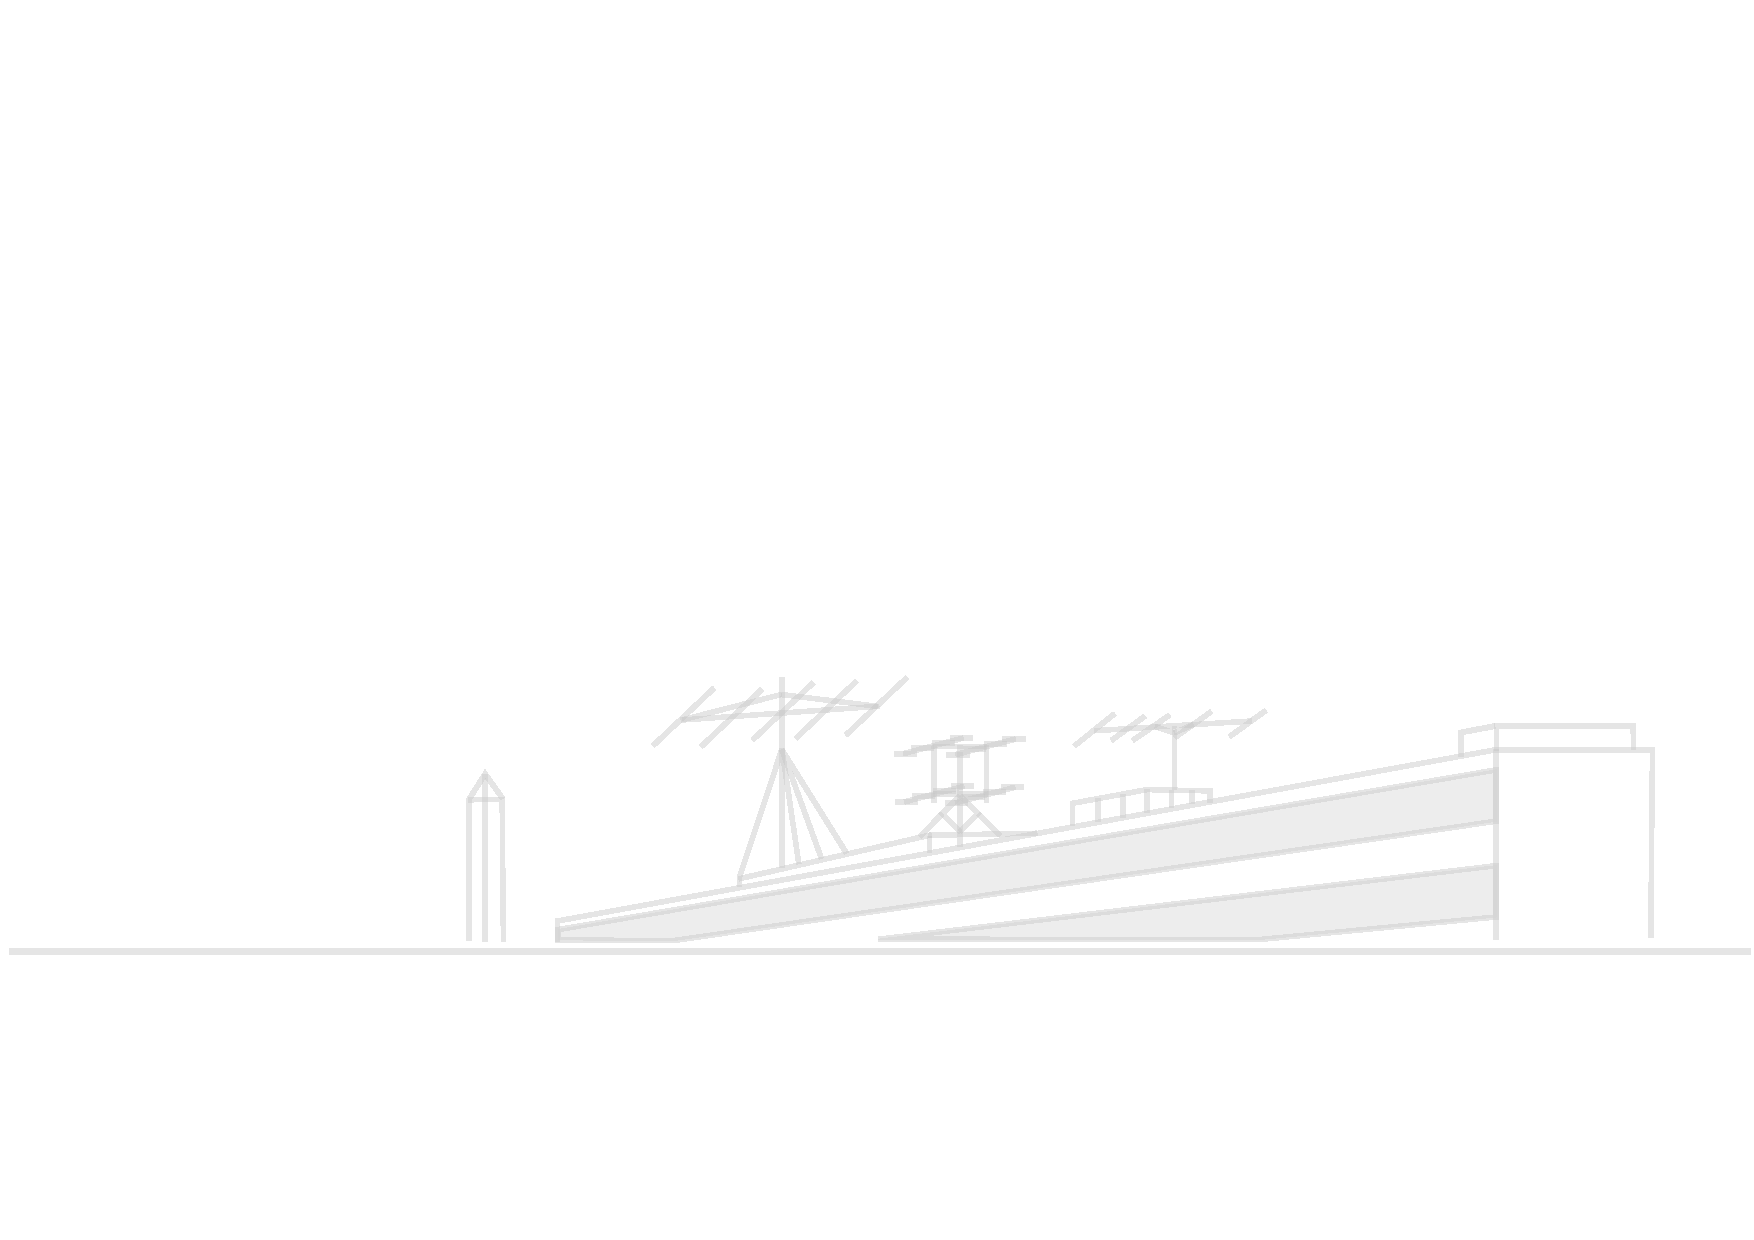
\includegraphics[width=17.8cm]{texdata/dk0tu_rooftop_background.pdf}
}

% Foliennummer einfügen
\setbeamertemplate{footline}[frame number]
%\setbeamertemplate{footline}{}

% Ändere das Zeichen vor jedem item
%\setbeamertemplate{itemize item}{\color{craneorange}$\blacktriangleright$}
%\setbeamertemplate{itemize subitem}{\color{craneorange}$\triangleright$}
%\setbeamertemplate{itemize subsubitem}{\color{craneorange}$\blacktriangleright$}

% Ändert die Blöcke 
\setbeamertemplate{blocks}[rounded][shadow=true]
% default | rounded [shadow=true|false]

%
% Eigene Kommandos
%

% Hack to get natbib and beamer working together. "The beamer user guide suggests
% that only the manual bibliography entry approach is supported"
% on some system it works out of the box, sometimes you need the hack :-(
% so check it --dl7bst
\ifdefined\newblock
    \relax
\else
    \newcommand{\newblock}{}
\fi

% \includedia command to generate png out of a dia file
% NEEDS installed dia and pdflatex option --shell-escape
\newcommand{\includedia}[1]{
    \immediate\write18{/usr/bin/dia #1.dia -e #1_diatmp.png -t png}
}

% RICHIG GROSSER FONT!
\newfont{\bigfont}{cmr10 at 144pt}
\newfont{\smallfont}{cmr10 at 8pt}

% Römische Ziffern
\makeatletter
\newcommand{\rmnum}[1]{\romannumeral #1}
\newcommand{\Rmnum}[1]{\expandafter\@slowromancap\romannumeral #1@}
\makeatother

% Schwarze Überschrift
%\setbeamercolor{frametitle}{fg=black}
%\setbeamercolor{title}{fg=black}

% Item- und Box-Farben
\definecolor{deepBlue}{HTML}{000066}
\setbeamercolor{itemize item}{fg=deepBlue}
\setbeamercolor{itemize subitem}{fg=deepBlue}
\setbeamercolor{description item}{fg=deepBlue}
\setbeamercolor{block title}{fg=deepBlue!100, bg=blue!15}
\setbeamercolor{block body}{fg=black, bg=blue!5}
\setbeamercolor{block title alerted}{fg=deepBlue, bg=red!75}
\setbeamercolor{block body alerted}{fg=black, bg=red!15}
\setbeamercolor*{block title example}{fg=blue!50, bg=blue!10}
\setbeamercolor*{block body example}{fg= blue, bg=blue!5}

%\setbeamercolor{section in head/foot}{parent=palette primary}
%\setbeamercolor{subsection in head/foot}{parent=palette secondary}
%\setbeamercolor{sidebar}{fg=darkblue,bg=yellow!90!orange}
%\setbeamercolor{title in sidebar}{fg=darkblue}
%\setbeamercolor{author in sidebar}{fg=darkblue}
%\setbeamercolor{section in sidebar}{fg=darkblue!10!black}
%\setbeamercolor{subsection in sidebar}{fg=darkblue!50!black}

% Titlepage Infos
\title{AFu-Kurs nach DJ4UF}
\author[DKØTU]{DKØTU\\ \footnotesize{Amateurfunkgruppe der TU Berlin}}
\institute[DKØTU]{\url{http://www.dk0tu.de} }

% PDF-Eigenschaften
\subject{DK0TU-Amateurfunkkurs nach DJ4UF}
\keywords{Amateurfunk Kurs HAM Radio Course CC-BY-NC-SA OpenSource TU Berlin DK0TU}

\subtitle{Technik 15: \\
  Sender- und Empfängertechnik \\[2em]}
\date{Stand 05.12.2016}
 \begin{document}

\begin{frame}
    \titlepage
    \vfill
    \begin{center}
        \ccbyncsaeu\\
        {\tiny This work is licensed under the \em{Creative Commons Attribution-NonCommercial-ShareAlike 3.0 License}.}\\[0.5ex]
         \tiny Amateurfunkgruppe der Technische Universität Berlin (AfuTUB), DKØTU
         %\includegraphics[scale=0.5]{img/DK0TU_Logo.pdf}
    \end{center}
\end{frame}


\section*{Einleitung}

\begin{frame}
  \frametitle{Was ist das?}
  \begin{center}
    \begin{figure}
      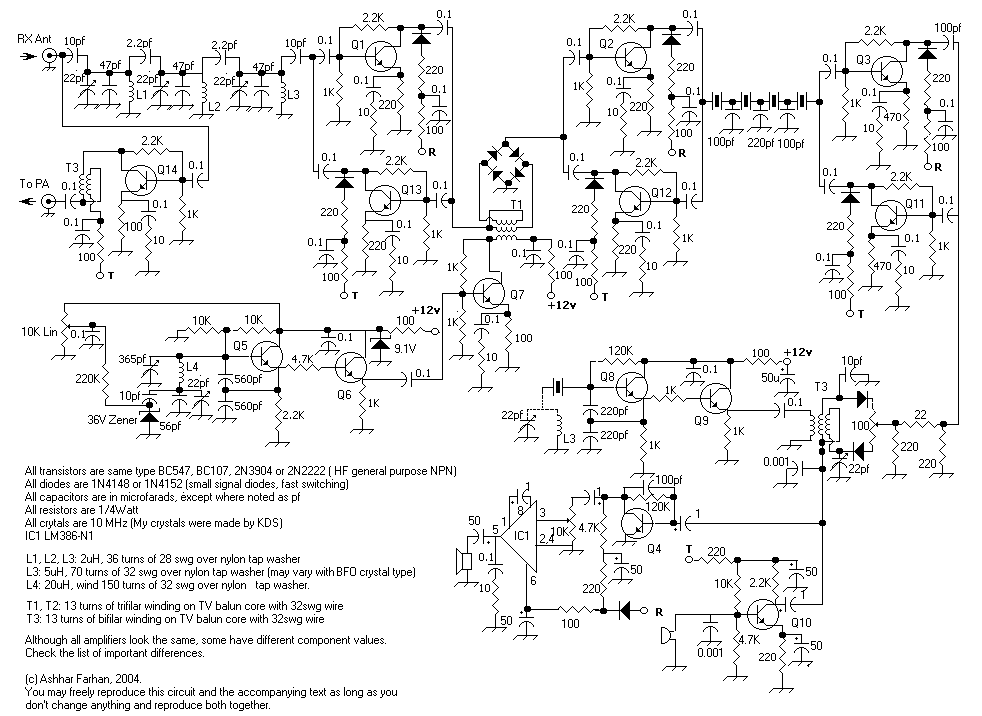
\includegraphics[width=.95\textwidth,height=.75\textheight,keepaspectratio]{e15/bitx.png}
      \caption{Schaltplan von \ExternalLink\url{http://www.phonestack.com/farhan/bitx.html}}
    \end{figure}
  \end{center}
\end{frame}

\begin{frame}
  \frametitle{In freier Wildbahn}
  \begin{itemize}
    \item Wo findet man Sender?
    \item Wo findet man Empfänger?
  \end{itemize}
\end{frame}

\begin{frame}
  \frametitle{Funktion}
  \begin{center}
    \begin{figure}
      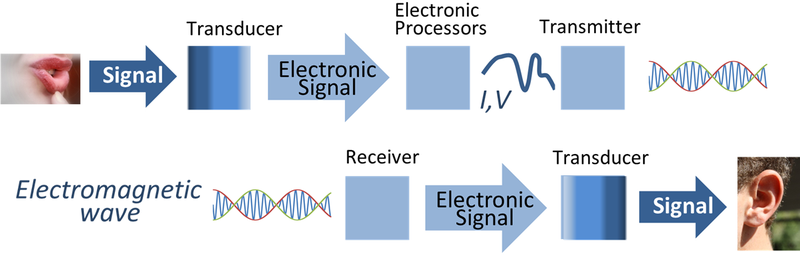
\includegraphics[width=1\textwidth,height=.75\textheight,keepaspectratio]{e15/TRX-superSimple.png}
      \attribcaption{Steps in a signal communications system}{Brews ohare}{https://en.wikipedia.org/wiki/File:Signal_processing_system.png}{\ccbysa}
    \end{figure}
  \end{center}
\end{frame}

\section*{Sender}

\begin{frame}
  \frametitle{Sender -- Blockschaltbild}
  \begin{center}
    \begin{figure}
      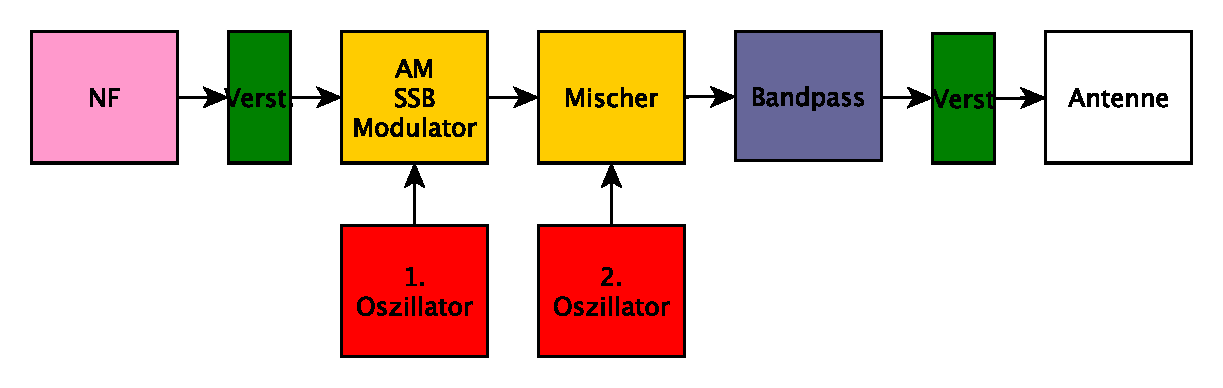
\includegraphics[width=1\textwidth,height=.75\textheight,keepaspectratio]{e15/ssb-trx-bsb.pdf}
      \caption{von DB4UM}
    \end{figure}
  \end{center}
\end{frame}

\begin{frame}
  \frametitle{Sender}
  \begin{center}
    \begin{figure}
      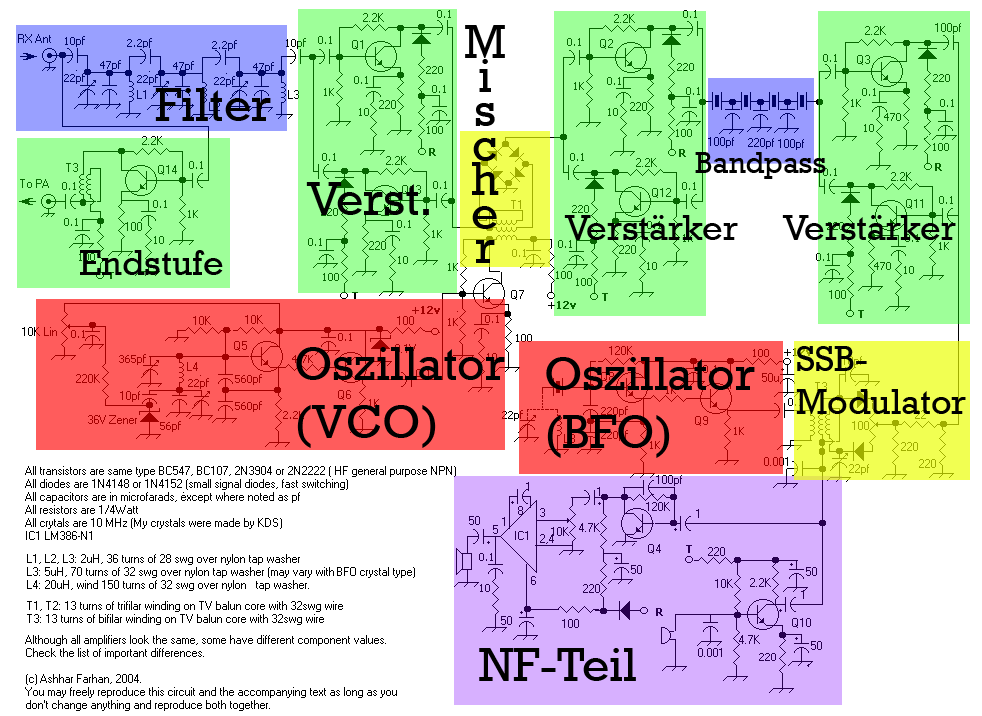
\includegraphics[width=.95\textwidth,height=.75\textheight,keepaspectratio]{e15/bitx-farbe.png}
      \caption{Schaltplan von \ExternalLink\url{http://www.phonestack.com/farhan/bitx.html}}
    \end{figure}
  \end{center}
\end{frame}

\begin{frame}
  \begin{center}
    \begin{figure}
      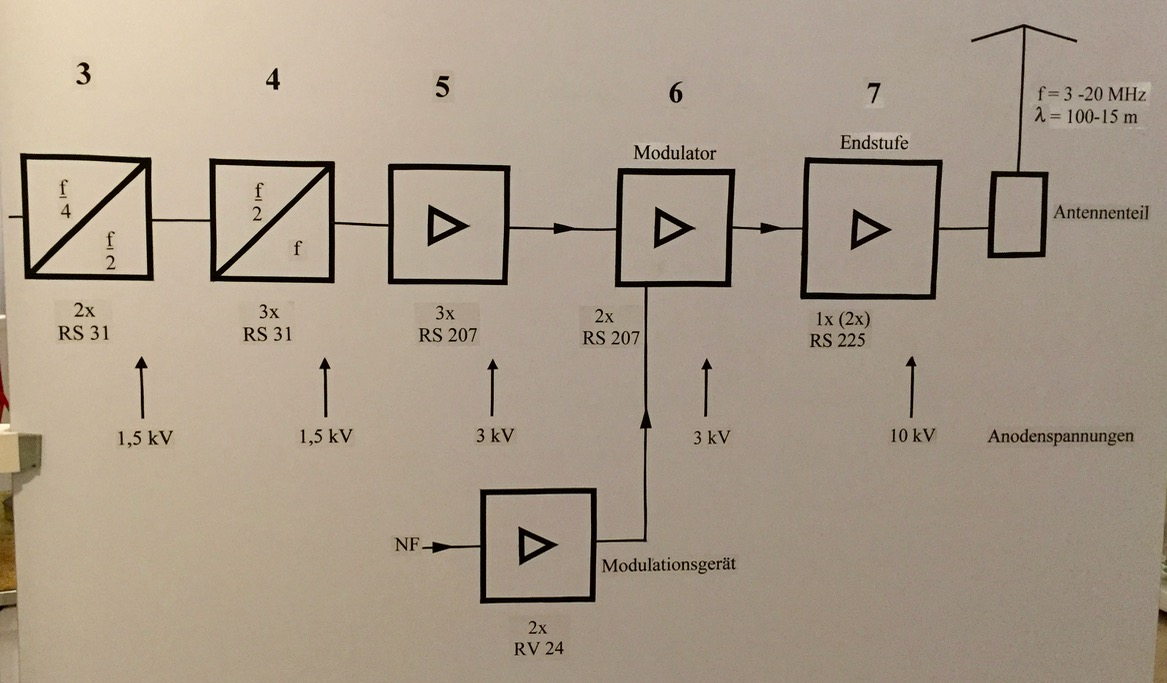
\includegraphics[width=1\textwidth,height=.8\textheight,keepaspectratio]{e15/Blockschaltbild_Runfunksender_Zeesen.jpg}
      \attribcaption{Blockschaltbild des Weltrundfunksenders Zeesen 1929 im Sender- und Rundfunkmuseum Königs Wusterhausen}{DC4LW (eigene Aufnahme)}{http://dc4lw.de}{}
    \end{figure}
  \end{center}
\end{frame}

\section*{Oszillator}

\begin{frame}
  \frametitle{Oszillator}
  \begin{center}
    \begin{itemize}
      \item VCO
        \begin{itemize}
          \item Voltage Controlled Oszillator
          \item Auch VFO (Variable Frequency Oszillator)
          \item Spannungsabhängiger Oszillator \\ ""
        \end{itemize}
      \item BFO
        \begin{itemize}
          \item Beat Frequency Oszillator
          \item Möglichst frequenzstabil auf einer Frequenz
        \end{itemize}
    \end{itemize}
  \end{center}
\end{frame}

%\begin{frame}
%  \frametitle{Prüfungsfrage}
%
%  \begin{center}
%    \begin{tabular}{l||p{.8\textwidth}}\hline
%      \textbf{TD604} & \textbf{Wie verhält sich die Frequenz eines LC-Oszillators bei Temperaturanstieg, wenn die Kapazität des Schwingkreiskondensators mit dem Temperaturanstieg geringer wird?} \\ \hline\hline
%      A & Die Frequenz wird niedriger. \\\hline
%      B & Die Frequenz bleibt stabil. \\\hline
%      C \only<2>\checkmark & Die Frequenz wird erhöht. \\ \hline
%      D & Die Schwingungen reißen ab (Aussetzer).\\\hline
%    \end{tabular}
%  \end{center}
%\end{frame}

\section*{Mischer}

\begin{frame}
  \frametitle{Mischer}
  \begin{center}
    \begin{figure}
      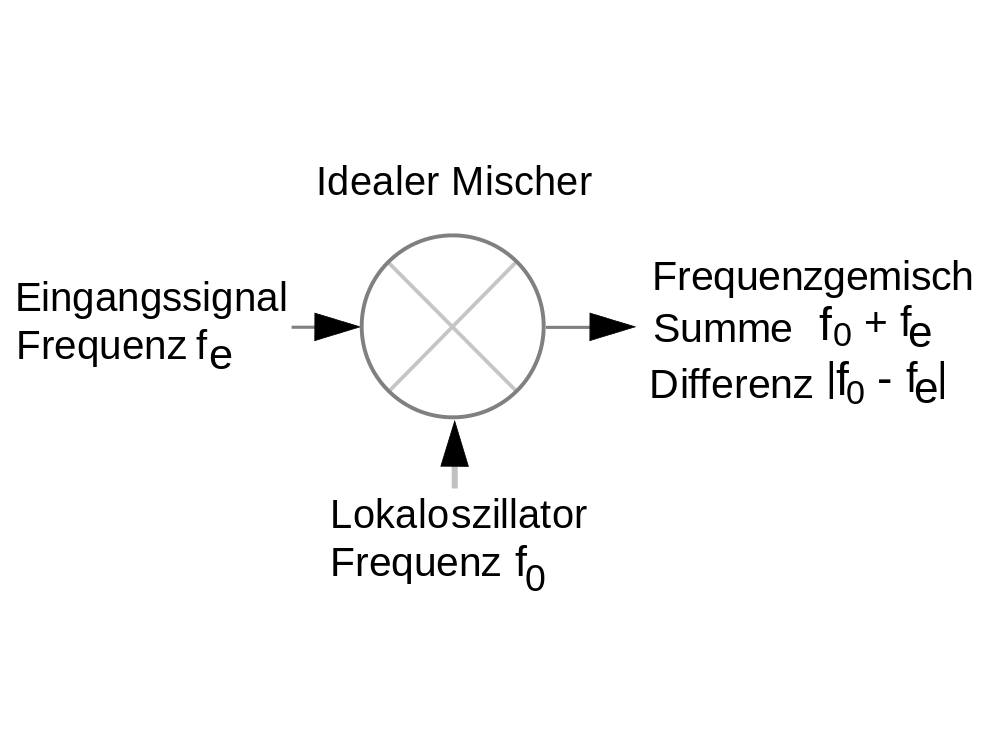
\includegraphics[width=.8\textwidth,height=.65\textheight,keepaspectratio]{e15/IdealerMischer.png}
      \attribcaption{Mischer}{Herbertweidner}{https://commons.wikimedia.org/wiki/File:Mischer.svg}{\ccPublicDomain}
    \end{figure}
  \end{center}
  Es fallen immer mehrere Frequenzen als Geschmisch heraus.
\end{frame}

\begin{frame}
  \frametitle{Realer Diodenmischer}
  \begin{center}
    \begin{figure}
      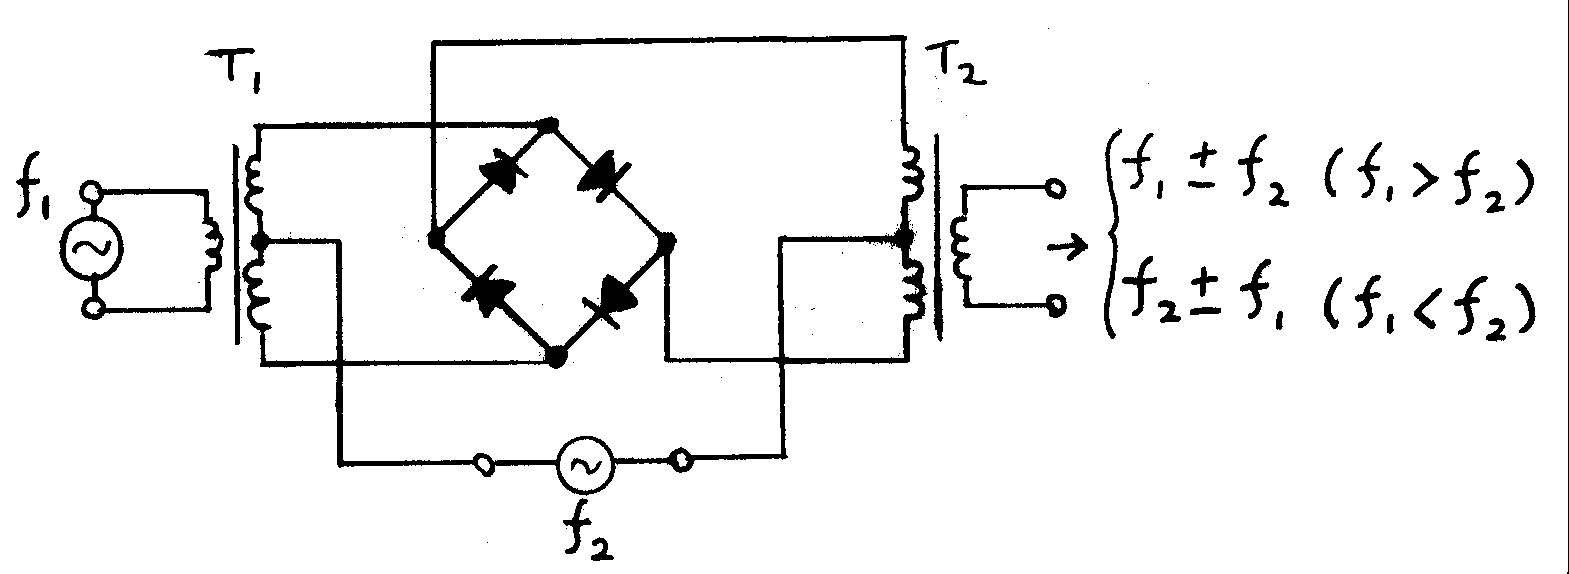
\includegraphics[width=.9\textwidth,height=.75\textheight,keepaspectratio]{e15/Realer-Diodenmischer.png}
      \attribcaption{Diodenmischer}{(japanische Zeichen nicht darstellbar)}{https://commons.wikimedia.org/wiki/File:Diode_DBM.png}{\ccbysa}
    \end{figure}
  \end{center}
\end{frame}

\begin{frame}
  \begin{exampleblock}{Mischer Rechenübung}
    \begin{itemize}
      \item Oszillator 1: $10 MHz$
      \item Oszillator 2: $4.1 MHz$
    \end{itemize}
    Welche Ausgangsfrequenzen?
  \end{exampleblock}
  \pause
  \begin{exampleblock}{Ergebnis}
    \begin{itemize}
      \item Ausgangsfrequenz 1: $14.1 MHz$
      \item Ausgangsfrequenz 2: $5.9 MHz$
    \end{itemize}
  \end{exampleblock}
\end{frame}

%\begin{frame}
%  \frametitle{Prüfungsfrage}
%
%  \begin{center}
%    \begin{tabular}{l||p{.8\textwidth}}\hline
%      \textbf{TF107} & \textbf{Einem Mischer werden die Frequenzen 28 MHz und 38,7 MHz zugeführt. Welche Frequenzen werden beim Mischvorgang erzeugt?}\\ \hline\hline
%      A & 10,7 MHz und 56 MHz \\\hline
%      B & 10,7 MHz \\\hline
%      C & 56 MHz und 66,7 MHz \\ \hline
%      D \only<2>\checkmark & 10,7 MHz und 66,7 MHz\\\hline
%    \end{tabular}
%  \end{center}
%  \pause
%  Hinweis: Die ungewollte Frequenz heißt auch Spiegelfrequenz.
%\end{frame}

\section*{Transverter}

\begin{frame}
  \frametitle{Transverter -- Blockschaltbild}
  Kofferwort: Transceiver + Konverter
  \begin{center}
    \begin{figure}
      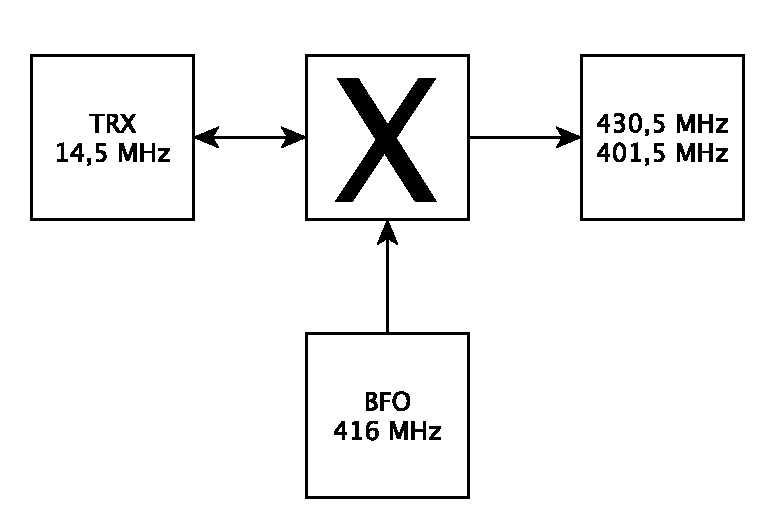
\includegraphics[width=1\textwidth,height=.6\textheight,keepaspectratio]{e15/transverter.pdf}
      \caption{Transverter}
    \end{figure}
  \end{center}
  Frequenzerweiterung für das Funkgerät. Hier: 20m auf 70cm.
\end{frame}

\section*{Empfänger}

\begin{frame}
  \frametitle{Direktüberlagerungsempfänger}
  Oder auch \emph{Superheterodynempfänger}, \emph{Superhet} oder \emph{Super}
  \begin{description}
    \item[super] \textit{(lat. super)} über
    \item[hetero] \textit{(griech. $\varepsilon\tau\varepsilon\rho o\varsigma$)} verschieden
    \item[dyn] \textit{(griech. $\delta\upsilon\nu\alpha\mu\iota\varsigma$)} Kraft
  \end{description}
  $\rightarrow$ Mischung zweier Signale unterschiedlicher Frequenz
\end{frame}

\begin{frame}
  \frametitle{Direktüberlagerungsempfänger -- Blockschaltbild}
  \begin{center}
    \begin{figure}
      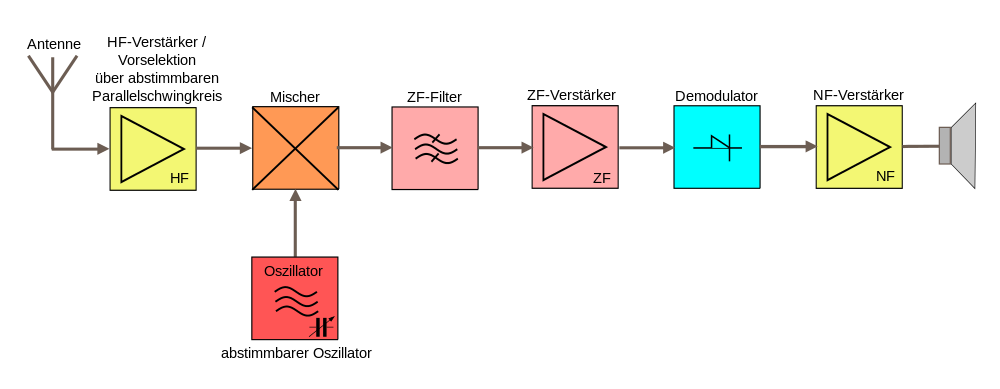
\includegraphics[width=.99\textwidth]{e15/Ueberlagerungsempfanger_blockschaltbild.png}
      \attribcaption{Überlagerungsempfänger}{Appaloosa}{https://commons.wikimedia.org/wiki/File:Ueberlagerungsempfanger_blockschaltbild.svg}{\ccbysa}
    \end{figure}
  \end{center}
\end{frame}

\begin{frame}
  \frametitle{Spiegelfrequenz}
  \begin{center}
    \begin{figure}
      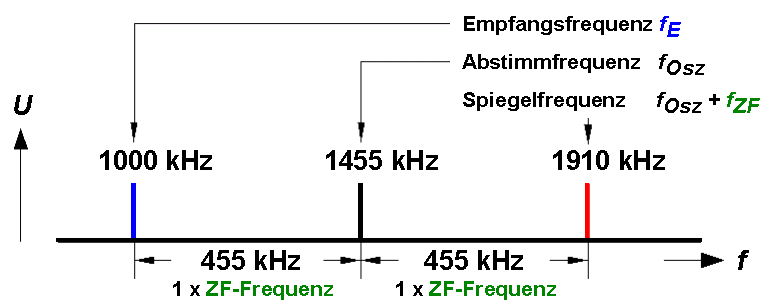
\includegraphics[width=.99\textwidth]{e15/Uberlagerungsempfanger_Spiegelfrequenz.png}
      \attribcaption{Spiegelfrequenz}{Znarf}{https://commons.wikimedia.org/wiki/File:Überlagerungsempfänger_Spiegelfrequenz.PNG}{\ccbysa}
    \end{figure}
  \end{center}
\end{frame}

\section*{Sonstiges}
\begin{frame}
  \frametitle{SNR}
  \begin{itemize}
    \item Das Signal-Rausch-Verhältnis dient als Bewertungszahl zur Beurteilung der Qualität eines (analogen) Kommunikationspfades.
    \item Um Sprache verstehen zu können braucht es ein SNR von ca 6dB.
  \end{itemize}
\end{frame}

\begin{frame}
  \frametitle{Trennschärfe}
  \begin{itemize}
    \item Beurteilt wie gut der Empfänger ein Signal von starken benachbarten Signalen trennen kann.
    \item Je steiler der Bandpass, desto besser die Trennschärfe.
  \end{itemize}
\end{frame}

\begin{frame}
  \frametitle{Großsignalfestigkeit}
  \begin{itemize}
    \item Beurteilt wie gut der Empfänger mit ganz starken Signalen zurechtkommt.
    \item Bekannt ist z.B. dann ein zugestopft des Empfängers bei zu starken Signalen (Erkennbar durch brummen).
  \end{itemize}
\end{frame}

\section*{Transceiver}

\begin{frame}
  \frametitle{BITX}
  \begin{figure}
    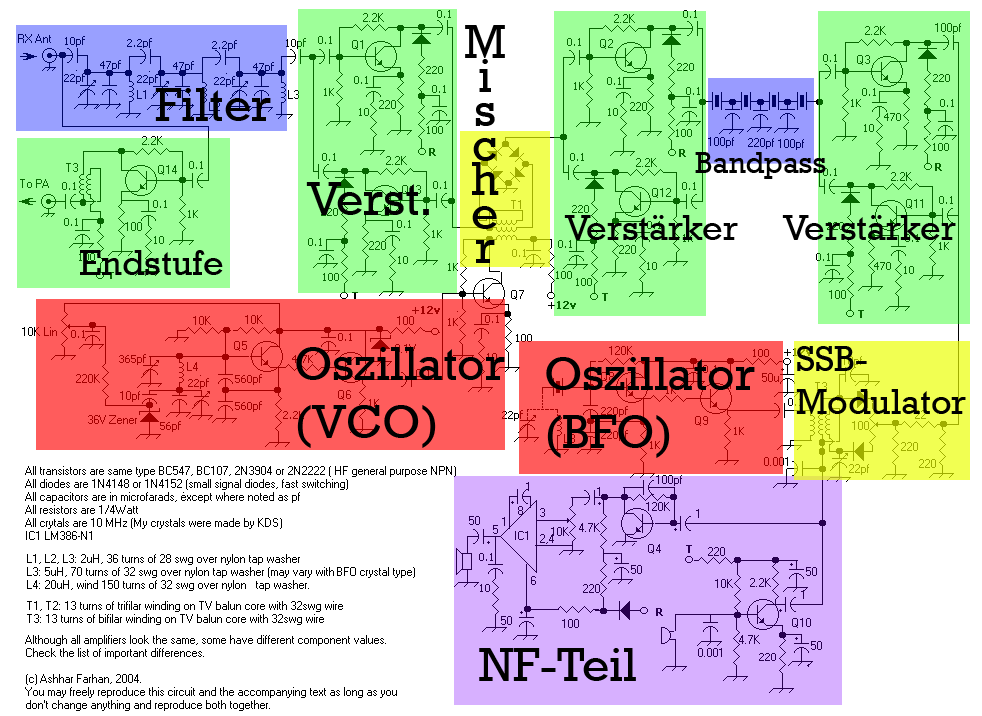
\includegraphics[width=.95\textwidth,height=.75\textheight,keepaspectratio]{e15/bitx-farbe.png}
      \caption{Schaltplan von \ExternalLink\url{http://www.phonestack.com/farhan/bitx.html}}
  \end{figure}
  6W SSB Transceiver für 14MHz
\end{frame}

\begin{frame}
  \frametitle{Elecraft - K3}
  \begin{center}
    \begin{figure}
      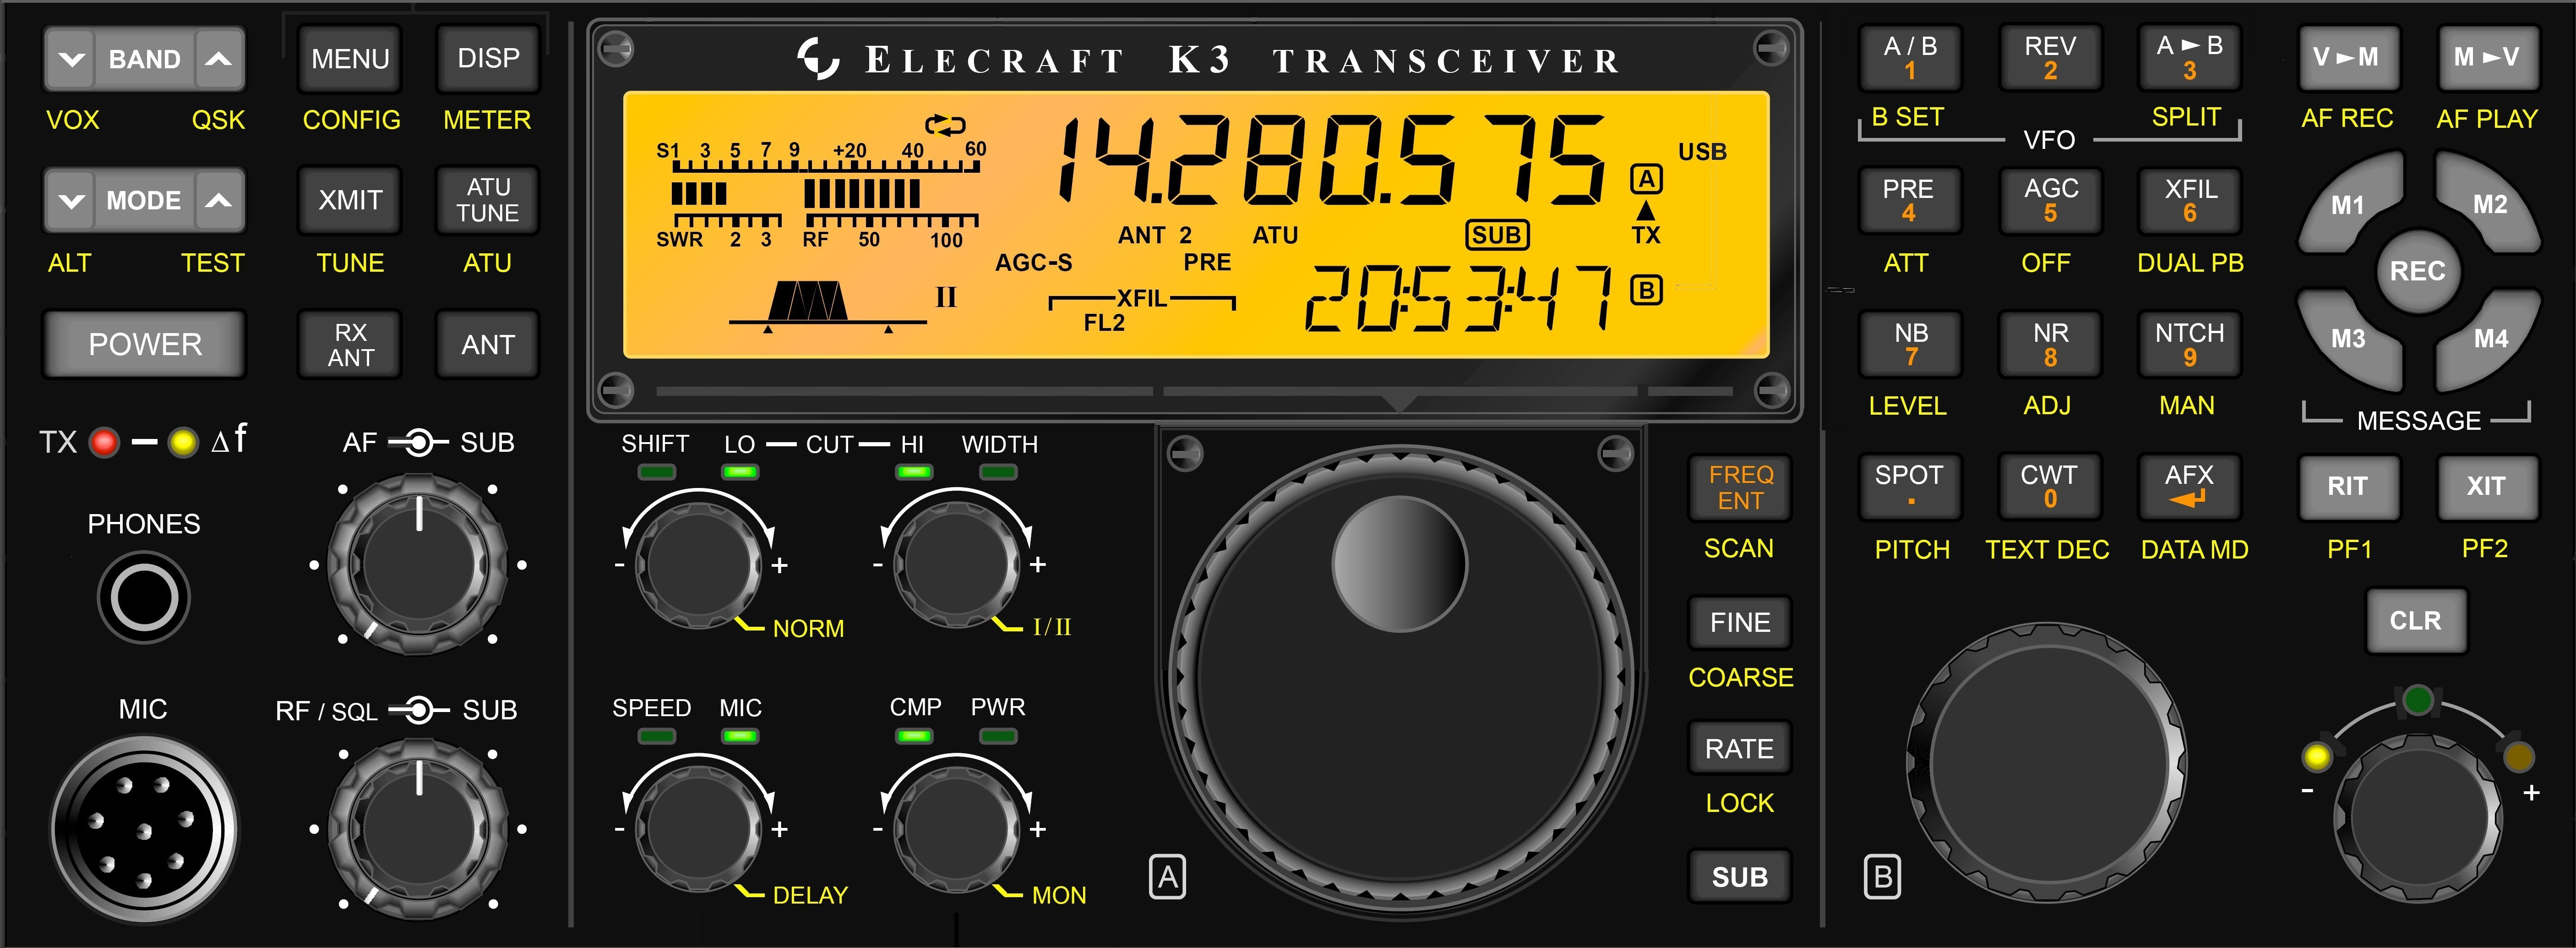
\includegraphics[width=1\textwidth,height=.75\textheight,keepaspectratio]{e15/K3_Front.jpg}
      \caption{Bild von \ExternalLink\url{http://www.elecraft.com/K3/K3.htm}}
    \end{figure}
  \end{center}
\end{frame}

\begin{frame}
  \frametitle{Drake TR-7}
  \begin{center}
    \begin{figure}
      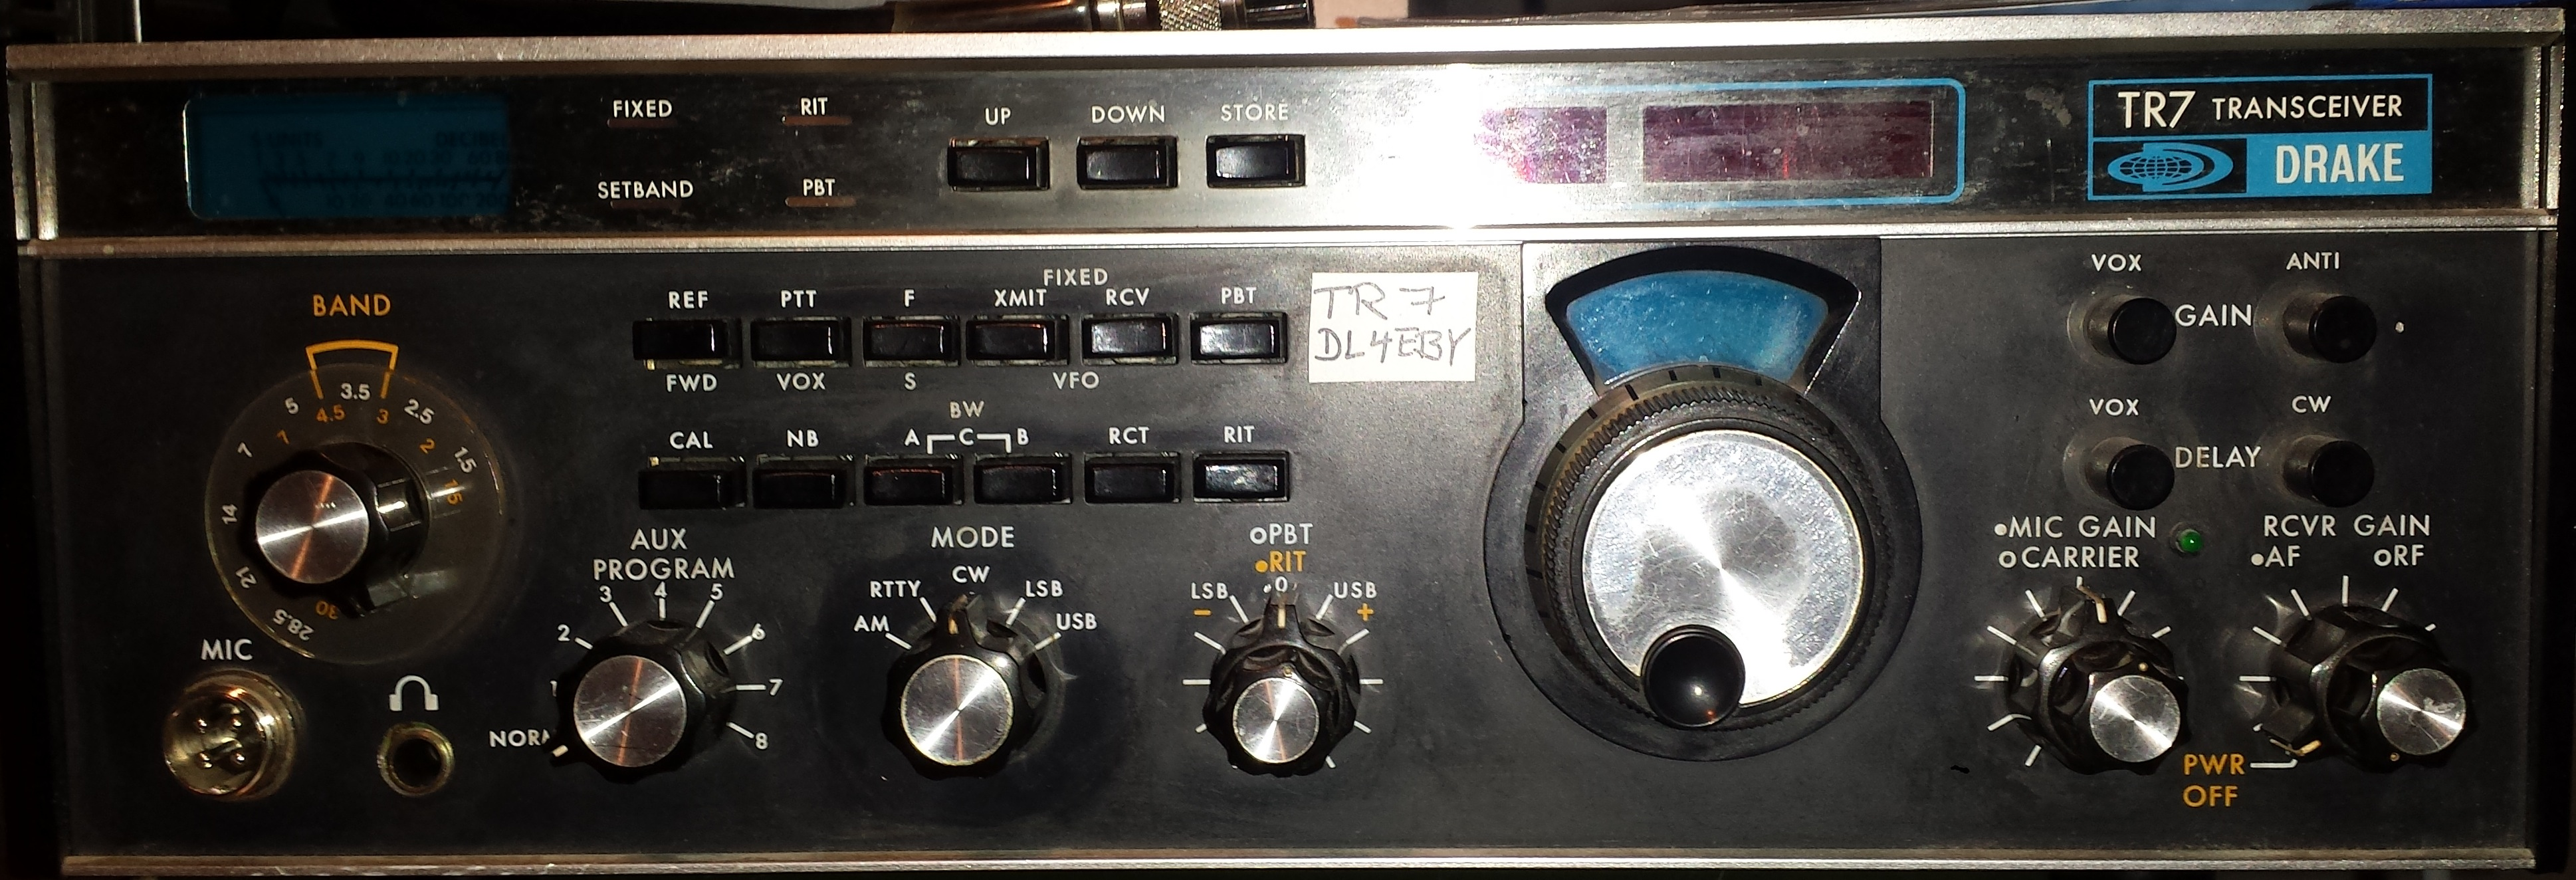
\includegraphics[width=1\textwidth,height=.75\textheight,keepaspectratio]{e15/drake.jpg}
      \caption{Bild von DB4UM bei DK0TU}
    \end{figure}
  \end{center}
\end{frame}

\begin{frame}
  \frametitle{rad1o}
  \begin{center}
    \begin{figure}
      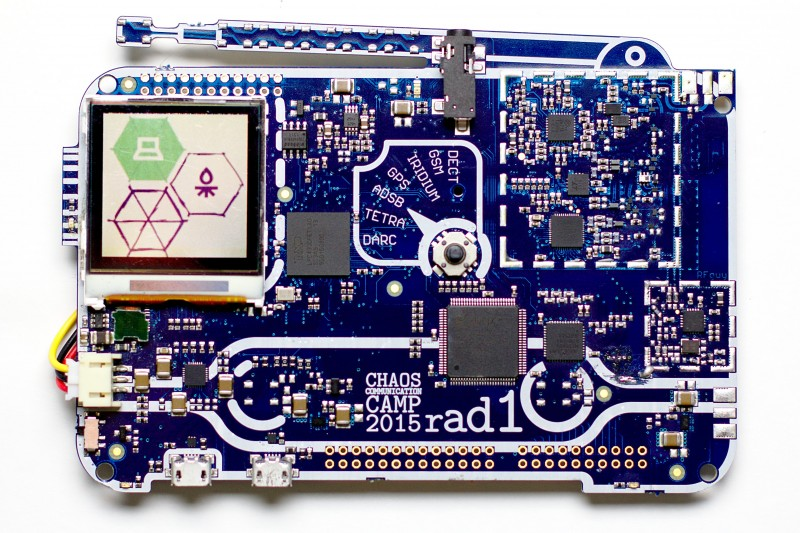
\includegraphics[width=1\textwidth,height=.75\textheight,keepaspectratio]{e15/rad1o.jpg}
      \caption{Bild von \ExternalLink\url{https://rad1o.badge.events.ccc.de/_media/rad1o_6.jpg}}
    \end{figure}
  \end{center}
\end{frame}

\begin{frame}
  \frametitle{rad1o -- Blockschaltbild}
  \begin{center}
    \begin{figure}
      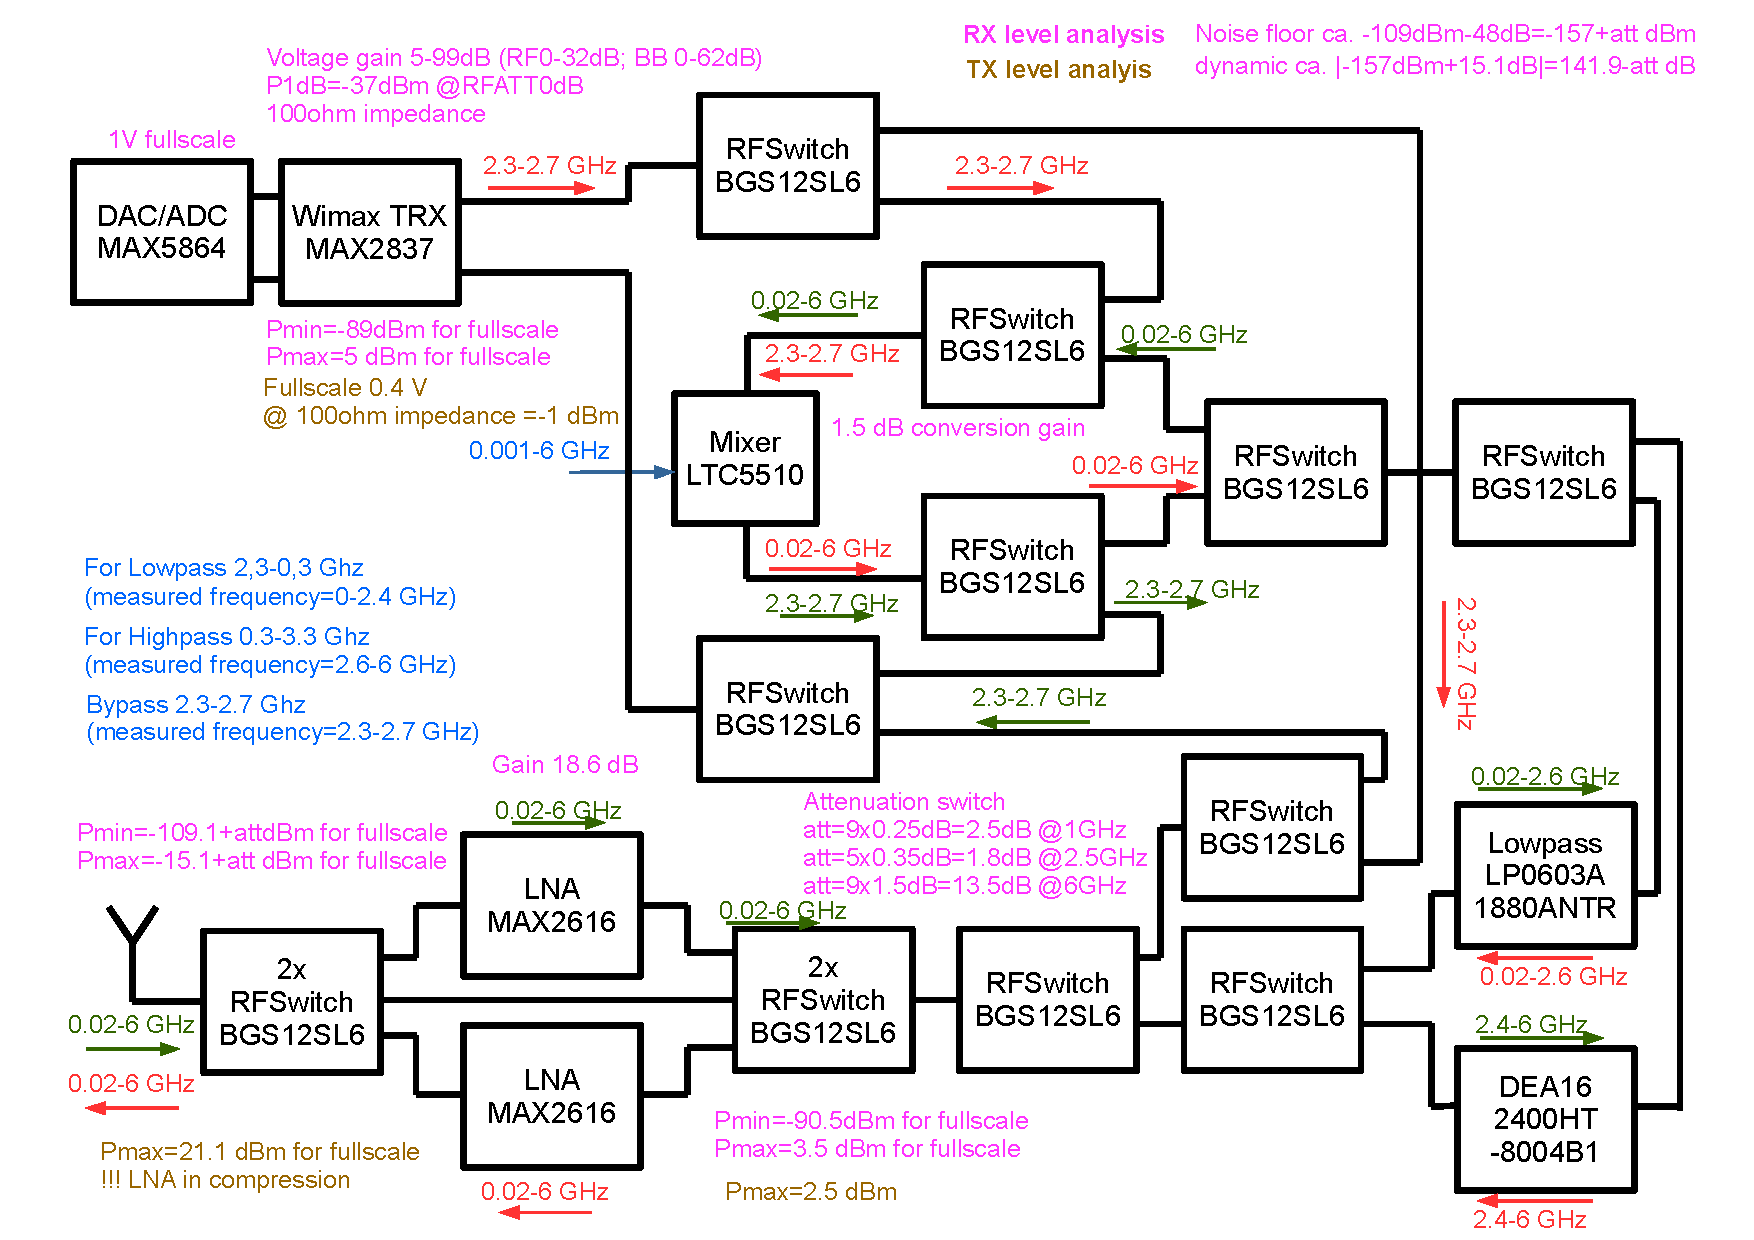
\includegraphics[width=1\textwidth,height=.75\textheight,keepaspectratio]{e15/rad1o_block.pdf}
      \caption{Schaltplan von \ExternalLink\url{https://github.com/rad1o/hardware/blob/master/concept/overview_RF.pdf}}
    \end{figure}
  \end{center}
\end{frame}

\section*{Referenzen}

\begin{frame}
  \frametitle{Referenzen/Links}

  \footnotesize
  \begin{itemize}
    \item Moltrecht E 15: \\
      \url{https://www.darc.de/der-club/referate/ajw/lehrgang-te/e15/}
    \item Überlagerungsempfänger (Wikipedia): \\
      \url{https://de.wikipedia.org/wiki/\%C3\%9Cberlagerungsempf\%C3\%A4nger}
  \end{itemize}

\end{frame}

% Hier könnte noch eine Kontaktfolie stehen

\end{document}

